%File: main_v5.tex  -- Nash Bargaining Preference Optimization (NBPO, pivot from RONPO)
\documentclass[letterpaper]{article} % DO NOT CHANGE THIS
\usepackage[submission]{aaai2027}  % DO NOT CHANGE THIS
\usepackage{times}  % DO NOT CHANGE THIS
\usepackage{helvet}  % DO NOT CHANGE THIS
\usepackage{courier}  % DO NOT CHANGE THIS
\usepackage[hyphens]{url}  % DO NOT CHANGE THIS
\usepackage{graphicx} % DO NOT CHANGE THIS
\urlstyle{rm} % DO NOT CHANGE THIS
\def\UrlFont{\rm}  % DO NOT CHANGE THIS
\usepackage{natbib}  % DO NOT CHANGE THIS
\usepackage{caption} % DO NOT CHANGE THIS
\frenchspacing  % DO NOT CHANGE THIS
\setlength{\pdfpagewidth}{8.5in} % DO NOT CHANGE THIS
\setlength{\pdfpageheight}{11in} % DO NOT CHANGE THIS
\usepackage{algorithm}
\usepackage{algorithmic}
\pdfinfo{/TemplateVersion (2026.1)}
\setcounter{secnumdepth}{0}
\usepackage{amsmath}
\usepackage{amssymb}
\usepackage{amsthm}
\usepackage{booktabs}
\usepackage{xcolor}

% float placement: discourage dedicated float pages
\setcounter{topnumber}{3}
\setcounter{dbltopnumber}{2}
\renewcommand{\topfraction}{0.92}
\renewcommand{\dbltopfraction}{0.92}
\renewcommand{\textfraction}{0.07}
\renewcommand{\floatpagefraction}{0.80}
\renewcommand{\dblfloatpagefraction}{0.80}

\newcommand{\revblue}{\color{blue}}
\newcommand{\note}[1]{\textcolor{red}{\textbf{[#1]}}}

% ============================================================================
% TODO: rebuttal experiment plan (priority order; none blocks submission).
% Local TODO(exp, ...) comments mark where each result lands in the text.
%   P0   LLM-scale covariance test (Theorem 3 at scale): noise one HH judge,
%        retrain all rules, report clean-surplus drift. Sole empirical axis
%        separating NBPO from maxmin on clean panels.
%   P0'  Nondegeneracy / conflict-regime diagnostic on the second panel.
%   P1   3 seeds + CIs, cross-judge evaluation, external benchmarks,
%        mean-length table.
%   P2   Published baselines: MaxMin-RLHF, MODPO, Rewarded Soups, RMOD.
%   P3   KS ideal-point split estimation; epsilon ablation; weight plots.
% Timeline: supplementary due Jul 31; Phase 1 notice Sep 24; author feedback
% Oct 19-25; final decision Nov 30. Target P0/P0'/P1 before Oct 19.
% MUST-FIX before submission: recheck page budget after the added lines.
% VERIFY against training logs: the stage-count numbers now consolidated in
% the appendix (NBS 0.749->0.833 with worst 0.710 at two stages; KS 0.867/0.773
% at four stages vs iterated averaging 0.859/0.755). The old Table 6 caption
% and the old appendix paragraph contradicted each other; the merged version
% assumes both sets of numbers are real.
% VERIFY: HT-MNPO naming. If the HT- prefix is our own variant of MNPO
% (wu2026mnpo), define the acronym once at first use.
% NOTE: figures/safe_radar.pdf is regenerated from the tab:lm2 values
% (make_safe_radar.py); restyle with the original plotting pipeline if
% desired. The retired uf_radar.pdf was the four-objective UltraFeedback
% radar and did not match the SafeRLHF caption.
% RESOLVED 2026-07-28: han2026fair metadata verified against arXiv:2602.04155
% (Han, Banerjee, Sun; submitted Feb 4, 2026; stat.ML).
% ============================================================================
\newtheorem{theorem}{Theorem}
\newtheorem{lemma}{Lemma}
\newtheorem{proposition}{Proposition}
\newtheorem{corollary}{Corollary}
\newtheorem{assumption}{Assumption}
\newtheorem{definition}{Definition}

\newcommand{\Y}{\mathcal{Y}}
\newcommand{\A}{\mathcal{A}}
\newcommand{\F}{\mathcal{F}}
\newcommand{\G}{\mathcal{G}}
\newcommand{\U}{\mathcal{U}}
\newcommand{\KL}{\mathrm{KL}}
\newcommand{\E}{\mathbb{E}}
\newcommand{\R}{\mathbb{R}}

\title{Nash Bargaining Preference Optimization}
\affiliations{}

\begin{document}
\maketitle

\begin{abstract}
Aligning a language model against $K$ conflicting preference judges forces a choice: a single policy ships, and it realizes one particular trade-off among the judges. Existing methods make this choice implicitly, either averaging the judges or maximizing the worst one. We make the choice itself the object of study. Anchoring judge $k$'s utility as the probability that it prefers the trained policy to the reference yields a bargaining problem whose disagreement point is known exactly: by skew-symmetry it is $\tfrac12$ in every coordinate. On this problem the classical axiomatic solutions of Nash and of Kalai and Smorodinsky become training objectives; the Nash one is our headline method, Nash Bargaining Preference Optimization (NBPO), and the Kalai--Smorodinsky one its individually monotone variant. Both provably serve every judge strictly better than the reference, are Pareto optimal, and are invariant to per-judge label noise, a covariance property that provably fails for both averaging and maxmin. Algorithmically the Nash objective dualizes into a bilinear saddle whose dual variables converge to the bargaining weights themselves; the method trains from binary comparisons alone and estimates nothing beyond $K$ win rates. On a controlled preference game these solutions raise every judge's anchored surplus above the reference where averaging drives one below it, and stay invariant to judge label noise where averaging and maxmin drift. On a four-judge language-model panel whose objectives genuinely conflict, the bargaining rules keep every judge near or above the reference where averaging drives the worst-off one well below it, giving the best worst-judge utility among methods that fix no target objective in advance; one round of the iteration makes the Kalai--Smorodinsky policy strictly better than the reference on all four judges. The separation holds across three independent evaluator families and closes, as the theory predicts, on a second panel whose judges do not conflict.
\end{abstract}

\section{Introduction}
Realistic alignment answers to several preference signals at once. Helpfulness, harmlessness, factuality, and domain critics judge the same model, and they disagree \citep{bai2022training,dai2024safe}. A single model ships, so alignment must commit to one point on the trade-off surface these judges span. The literature makes this commitment silently. Averaging methods collapse the judges into a fixed mixture and optimize its win rate \citep{wu2025sppo,zhang2025iterative}; maxmin methods harden the worst objective \citep{chakraborty2024maxmin,son2026rmod}; per-player formulations give each judge its own player, leaving the two-player class where last-iterate convergence is understood \citep{wu2026mnpo}. None asks which point a deployed policy should target, or why.

We take the selection problem as primary. The right language for it is cooperative bargaining: given a feasible set of jointly achievable outcomes and a status quo, which single outcome should $K$ parties agree on? Bargaining theory answers this axiomatically, and its two classical solutions, due to \citet{nash1950} and to \citet{kalai1975}, are characterized by exactly the properties an alignment designer wants: invariance to how each judge is scaled, no judge left below the status quo, and stability under changes to the option set. We show these solutions are computable as alignment objectives, prove the guarantees they inherit, and give a practical iterative preference optimization algorithm.

The construction rests on one modeling choice that removes the usual estimation burden. If alignment fails, the reference model ships unchanged, so a judge's utility should be measured against the reference and the utility of shipping the reference should be the status quo. Anchoring the utility of a policy $\pi$ at the average probability $u_k(\pi)=P_k(\pi\succ\mu)$ that judge $k$ prefers $\pi$ to the reference $\mu$ makes this exact: by skew-symmetry of preference, $u_k(\mu)=\tfrac12$ for every judge, so the disagreement point is $\tfrac12\mathbf 1$ with no estimation. This same anchoring makes each utility linear in the policy, which is what lets the method train from binary comparisons alone.

Our contributions are: (i) the anchored bargaining formulation of multi-judge alignment, with an exactly known disagreement point, and Nash Bargaining Preference Optimization (NBPO), the training objective it induces; (ii) a guarantee package, individual rationality, Pareto optimality, and a covariance property that separates bargaining from both averaging and maxmin; (iii) a primal--dual algorithm whose dual variables are the bargaining weights and whose policy update is a single squared-loss regression on binary labels, estimating nothing beyond $K$ win rates, with a linear last-iterate convergence guarantee; and (iv) a controlled-game validation of the individual-rationality and covariance guarantees, and a language-model panel on which the bargaining rules separate from averaging on worst-judge utility, under three independent evaluators and without fixing a target objective in advance, with a second panel showing the advantage is confined to genuine conflict.

\section{Background}
\paragraph{Preference-based alignment.}
We work in the preference-based contextual bandit that underlies RLHF \citep{yue2012karmed,dudik2015contextual}. A prompt $x$ is drawn from $\rho$; a policy maps $x$ to a distribution $\pi(\cdot\mid x)$ over a finite response set $\Y$; and feedback is relative. A preference oracle $P:\Y\times\Y\times\mathcal{X}\to[0,1]$ returns the probability that one response is preferred to another, and is skew-symmetric,
\begin{equation}
P(y\succ y'\mid x)+P(y'\succ y\mid x)=1,\quad P(y\succ y\mid x)=\tfrac12 .
\label{eq:skew}
\end{equation}
The oracle need not come from a scalar utility, so cyclic preferences are allowed \citep{may1954intransitivity}. For policies, $P(\pi\succ\pi'\mid x)=\E_{y\sim\pi,y'\sim\pi'}[P(y\succ y'\mid x)]$. We fix a context and drop $x$; every statement lifts by conditioning and averaging. Nash learning from human feedback \citep{munos2024nash,azar2024general} seeks a von Neumann winner through the KL-regularized game $\max_\pi\min_{\pi'}P(\pi\succ\pi')-\tau\KL(\pi\|\mu)+\tau\KL(\pi'\|\mu)$, and INPO \citep{zhang2025iterative} turns each mirror step into a regression on pairwise log-ratios that needs only binary outcomes. Alignment with $K$ oracles $P_1,\dots,P_K$ is the setting of interest; the question is what to do when they conflict.

\paragraph{Bargaining problems.}
A $K$-player bargaining problem is a pair $(\F,d)$ where $\F\subset\R^K$ is compact and convex, $d\in\F$, the set is comprehensive relative to $d$, and some $u\in\F$ has $u>d$ componentwise. A solution $f$ assigns to every such problem a point $f(\F,d)\in\F$. Coordinate $k$ of $u\in\F$ is the utility judge $k$ receives; $d$ is the disagreement point.
\citet{nash1950} proposed four axioms: Pareto optimality (PO), symmetry (SYM), scale covariance (SC, invariance to positive affine rescaling of any coordinate), and independence of irrelevant alternatives (IIA). Exactly one solution satisfies all four:
\begin{equation}
f^{\mathrm N}(\F,d)=\arg\max_{u\in\F,\,u>d}\;\sum_{k=1}^{K}\log(u_k-d_k).
\label{eq:nash}
\end{equation}
The log form weights judge $k$'s direction by $1/(u_k-d_k)$, the inverse of its realized surplus, so the judge closest to walking away speaks loudest while no judge's gain is traded to exactly zero. \citet{kalai1975} replace IIA by individual monotonicity (IM): an expansion that leaves the other judges' best hopes untouched must not hurt a judge. With the ideal point $u^\ast_k=\max\{u_k:u\in\F,u\ge d\}$, their solution is the maximal feasible point on the segment from $d$ to $u^\ast$, equivalently
\begin{equation}
f^{\mathrm{KS}}(\F,d)\in\arg\max_{u\in\F}\;\min_k\frac{u_k-d_k}{u^\ast_k-d_k},
\label{eq:ks}
\end{equation}
a maximin over canonically normalized surpluses. Throughout, Nash names the bargaining solution \eqref{eq:nash} and not the equilibrium of a two-player preference game, the object targeted by Nash learning from human feedback. Table~\ref{tab:axioms} records how the four candidate rules fare on this domain; NBS and KS are the only two keeping PO, SYM, and SC, and they part ways only on IIA versus IM.

\begin{table}[t]
\centering\footnotesize
\setlength{\tabcolsep}{3.5pt}
\begin{tabular}{lccccc}
\toprule
Rule & PO & SYM & SC & IIA & IM \\
\midrule
Utilitarian $\max\sum_k u_k$ & \checkmark & \checkmark & $\times$ & \checkmark & $\times$ \\
Egalitarian $\max\min_k(u_k{-}d_k)$ & weak & \checkmark & $\times$ & \checkmark & \checkmark \\
Nash (NBS) & \checkmark & \checkmark & \checkmark & \checkmark & $\times$ \\
Kalai--Smorodinsky (KS) & \checkmark & \checkmark & \checkmark & $\times$ & \checkmark \\
\bottomrule
\end{tabular}
\caption{Axiom satisfaction of the four selection rules. The utilitarian rule is averaging; the egalitarian rule is maxmin. Only NBS and KS keep scale covariance.}
\label{tab:axioms}
\end{table}

\section{Alignment as a Bargain Among Judges}
\label{sec:bargain}
The players are the $K$ judges. The design question is what a judge's utility should be, and we resolve it through the disagreement point. If alignment fails, the reference $\mu$ ships, so a judge's utility is measured against $\mu$.

\begin{definition}[Anchored utility and surplus]
For a policy $\pi$ and judge $k$,
\begin{equation}
\begin{aligned}
u_k(\pi)&=P_k(\pi\succ\mu)=\textstyle\sum_y\pi(y)\,m_k(y),\\
s_k(\pi)&=u_k(\pi)-\tfrac12,
\end{aligned}
\label{eq:anchor}
\end{equation}
with $m_k(y)=\E_{y'\sim\mu}P_k(y\succ y')$ the margin of $y$ over $\mu$.
\end{definition}

The surplus $s_k(\pi)$ is the average margin by which judge $k$ favors $\pi$ over $\mu$: positive means the judge prefers the trained model.

\begin{lemma}[Structure]
\label{lem:struct}
Each $u_k$ is linear in $\pi$ with values in $[0,1]$; the disagreement point is exact, $u_k(\mu)=\tfrac12$ for every $k$, so $d=\tfrac12\mathbf 1$ with no estimation; and the feasible set $\U=\{u(\pi):\pi\in\Delta(\Y)\}$ is a compact convex polytope containing $d$, whose comprehensive hull paired with $d$ is a bargaining problem whenever some policy beats $\mu$ under every judge at once.
\end{lemma}

Three remarks. First, the disagreement point being exact is not cosmetic: bargaining solutions are sensitive to $d$, and any estimated $d$ propagates its error into the selected point; here skew-symmetry pins $d$ analytically. Second, anchoring buys linearity, which the algorithm below converts into training whose only estimated objects are $K$ win rates. Third, anchoring fixes $\mu$ as the standing opponent, so every objective below depends on $P_k$ only through the margins $m_k$; cyclic structure among the policy's own responses never enters. What the oracle's generality buys is the interface: no reward model is fit, and $d$ is exact under skew-symmetry alone. The difficulty this paper addresses is the selection among judges, not the duel within one.

\begin{assumption}[Nondegeneracy]
\label{ass:nondeg}
Some $\pi$ has $s(\pi)>0$ componentwise. If nondegeneracy fails, $\mu$ is already weakly Pareto optimal and a leximin fallback applies.
\end{assumption}

\paragraph{What existing methods select.}
Every method that ships one policy selects one point of $\U$. Averaging solves the Nash game of a fixed mixture oracle $P_w=\sum_k w_kP_k$; since $P_w$ is skew-symmetric, that game has value exactly $\tfrac12$ whatever the conflict, so an averaged win rate near $\tfrac12$ certifies nothing about any individual judge. In outcome space averaging is the utilitarian corner $\max\sum_k w_ku_k$, which we show below can serve a judge strictly worse than the untrained reference. Maxmin selects the egalitarian corner $\max\min_k s_k(\pi)$, which is individually rational but, lacking scale covariance, changes selection when one judge's labels merely get noisier.

\paragraph{The bargaining objectives.}
For $\tau\ge0$ the Nash-bargained policy $\pi^{\mathrm N}_\tau$ and Kalai--Smorodinsky-bargained policy $\pi^{\mathrm{KS}}_\tau$ maximize
\begin{equation}
J^{\mathrm N}_\tau(\pi)=\sum_{k=1}^{K}\log s_k(\pi)-\tau\KL(\pi\|\mu),
\label{eq:jn}
\end{equation}
\begin{equation}
J^{\mathrm{KS}}_\tau(\pi)=\min_k\frac{s_k(\pi)}{u^\ast_k-\tfrac12}-\tau\KL(\pi\|\mu),
\label{eq:jks}
\end{equation}
respectively, with $u^\ast_k$ the anchored ideal. Both objectives are concave: $s_k$ is affine, log of a positive affine function is concave, a minimum of concave functions is concave, and $-\tau\KL$ is strongly concave, so $\pi^{\mathrm N}_\tau$ is unique. There is no saddle to compute and no inner adversary: the conflict among judges lives entirely in the curvature of one concave objective. For $K=1$ both reduce to the familiar one-step improvement objective $P(\pi\succ\mu)-\tau\KL(\pi\|\mu)$.

\section{Guarantees}
\label{sec:guarantees}
All proofs, with explicit constants and witness instances, are in the appendix.
\begin{theorem}[Individual rationality]
\label{thm:ir}
Under Assumption~\ref{ass:nondeg}: (i) for every $\tau\ge0$, $s_k(\pi^{\mathrm N}_\tau)>0$ for all $k$, so every judge strictly prefers the Nash-bargained policy to the reference; (ii) for every $\tau\ge0$, $s_k(\pi^{\mathrm{KS}}_\tau)>0$ for all $k$, with an explicit positive floor on the normalized surpluses; and (iii) the utilitarian (averaging) rule fails individual rationality: there are $K$-judge instances on which it selects a policy with $s_k<0$ for some judge.
\end{theorem}
The log barrier of the Nash product does the work at every regularization strength, so strict individual rationality is not a small-$\tau$ property. Part (iii) upgrades the hidden-objective collapse of averaging from an anecdote to an axiom violation on a certified instance. Both positive parts speak of the exact maximizer over $\Delta$; a parametric policy trained for finitely many stages inherits them up to optimization and estimation error, so surpluses near zero can survive training when nondegeneracy is marginal (see the Experiments).

\begin{theorem}[Pareto optimality]
\label{thm:po}
Under Assumption~\ref{ass:nondeg}, $\pi^{\mathrm N}_0$ is Pareto optimal in $(u_1,\dots,u_K)$, and for $\tau>0$, $\pi^{\mathrm N}_\tau$ is Pareto optimal in the extended vector $(u_1,\dots,u_K,-\KL(\cdot\|\mu))$; the Nash welfare loss from regularization is at most linear in $\tau$.
\end{theorem}

\begin{theorem}[Covariance to judge noise]
\label{thm:cov}
Degrading judge $k$ by replacing a fraction $1-\lambda_k$ of its labels with coin flips gives the skew-symmetric oracle $P^\lambda_k=\lambda_kP_k+(1-\lambda_k)\tfrac12$. Under this compression: (i) anchored surpluses rescale exactly, $s^\lambda_k=\lambda_ks_k$, while $d$ and the KL term are unchanged, and the ideals rescale the same way; (ii) both bargaining solutions are invariant, $\pi^{\mathrm N}_\tau$ and $\pi^{\mathrm{KS}}_\tau$ are unchanged for every $\lambda\in(0,1]^K$ and $\tau\ge0$; (iii) the utilitarian and egalitarian rules are not invariant and change their selected policy under some $\lambda$.
\end{theorem}
Operationally, if one judge becomes noisier, a maxmin-aligned model drifts toward the degraded judge and an averaging-aligned model also moves, while a bargained model does not. To our knowledge this is the first alignment-level consequence extracted from the scale covariance axiom, and it is directly testable.
% TODO(exp, P0): LLM-scale analogue of Table tab:cov. Inject label noise
% (lambda = 0.3) into one HH judge, retrain all four rules, report the drift
% of the clean surplus. This is the only empirical axis that separates NBPO
% from the egalitarian rule on clean panels; run before author feedback
% (Oct 19-25) and cite the numbers in the response.

\section{An Estimation-Free Algorithm}
\label{sec:algo}
The algorithm is a squared-loss regression on binary comparisons whose population minimizer coincides with the exact mirror update. Estimation-free means that no reward model, value function, or disagreement point is ever fit; the only estimated quantities in the method are the $K$ scalar win rates the weights consume.

\paragraph{Anatomy of the update.}
For a fixed weight vector $\omega\in\Delta(K)$ the weighted anchored objective $\sum_k\omega_ku_k(\pi)-\tau\KL(\pi\|\mu)$ is linear in $\pi$, its opponent is the fixed reference $\mu$, and its mirror step has the closed form \eqref{eq:closed} below, with reward $r(y)=\sum_k\omega_km_k(y)$. The corresponding regression target is $\sum_k\omega_kz_k$ with per-judge binary labels
\begin{equation}
z_k=\mathbf 1[y\succ_k y'']-\mathbf 1[y'\succ_k y''],\qquad y''\sim\mu,
\label{eq:target}
\end{equation}
one shared reference opponent for all judges. So the only obstruction the Nash rule adds is the weights themselves: the first-order condition weights judge $k$ by $1/s_k$, a nonlinear function of an expectation. No estimator built from finitely many binary comparisons is unbiased for $1/s_k$, so the nonlinearity must move either into $K$ estimated scalars or into optimizer state.

\paragraph{Primal--dual form.}
The Fenchel identity for the logarithm, $\log s=\min_{\lambda>0}(\lambda s-\log\lambda-1)$, relocates the weight into a dual variable and turns the Nash program into the bilinear saddle
\begin{equation}
\max_{\pi}\;\min_{\lambda>0}\;\sum_{k}\big(\lambda_ks_k(\pi)-\log\lambda_k-1\big)-\tau\KL(\pi\|\mu).
\label{eq:saddle}
\end{equation}
The coupling $\sum_k\lambda_ks_k(\pi)$ is bilinear, so the policy update at fixed $\lambda$ is exactly the weighted optimization step, and the dual optimum at fixed $\pi$ is $\lambda_k=1/s_k(\pi)$, the bargaining weight itself. The dual variable is not an adversary; its fixed point is the inverse-surplus bargaining vector, and the saddle is a benign bilinear coupling between two strongly regularized players, which is why plain mirror ascent reaches it at a linear last-iterate rate with no optimism or extragradient step (Proposition~\ref{prop:conv}).

\paragraph{From saddle to regression.}
Freeze the dual at its best response to the current policy, $\omega_{t,k}=1/s_k(\pi_t)$; normalizing these weights to the simplex, as the algorithm does, only rescales the step size $\eta_t$. One mirror-ascent step on \eqref{eq:saddle}, with the regularizer kept exact rather than linearized, is
\begin{equation}
\begin{aligned}
\pi_{t+1}=\arg\max_{\pi}\;&\eta_t\textstyle\sum_k\omega_{t,k}s_k(\pi)\\
&-\eta_t\tau\KL(\pi\|\mu)-\KL(\pi\|\pi_t).
\end{aligned}
\label{eq:md}
\end{equation}
Because $\sum_k\omega_{t,k}m_k$ is the gradient of $\sum_k\log s_k$ at $\pi_t$, the same step is Bregman proximal ascent on $J^{\mathrm N}_\tau$ itself (Lemma~\ref{lem:equiv}): the saddle and the concave program prescribe one iterate. Its closed form is the exponential tilt
\begin{equation}
\pi_{t+1}(y)\propto\Big(\pi_t(y)\,\mu(y)^{\eta_t\tau}\,e^{\eta_t\sum_k\omega_{t,k}m_k(y)}\Big)^{\!1/(1+\eta_t\tau)}.
\label{eq:closed}
\end{equation}
Log-ratios of \eqref{eq:closed} at a pair of responses eliminate the normalizer. Define
\begin{equation}
\begin{aligned}
h_t(\pi;y,y')&=\log\tfrac{\pi(y)}{\pi_t(y)}-\log\tfrac{\pi(y')}{\pi_t(y')}\\
&\quad+\eta_t\tau\Big(\log\tfrac{\pi(y)}{\mu(y)}-\log\tfrac{\pi(y')}{\mu(y')}\Big);
\end{aligned}
\label{eq:h}
\end{equation}
then the tilt \eqref{eq:closed} is the unique full-support policy $\pi$ satisfying $h_t(\pi;y,y')=\eta_t\sum_k\omega_{t,k}\{m_k(y)-m_k(y')\}$ at every pair, and that right side is the conditional mean of the observable target $\eta_t\sum_k\omega_{t,k}z_k$ of \eqref{eq:target}. Squared loss turns a conditional mean into a population minimizer, which closes the chain from \eqref{eq:jn} to the loss in Algorithm~\ref{alg:nbpo}.
\begin{proposition}[The regression is the mirror step]
\label{prop:exact}
Fix any weights $\omega_t\in(0,\infty)^K$, let $\pi_t$ and $\mu$ have full support, and let $\pi_{t+1}$ be \eqref{eq:closed} under these weights. Draw $y,y'\sim\pi_t$ and $y''\sim\mu$ independently with binary labels of mean $P_k$. Over full-support policies, the population minimizer of $\E\big(h_t(\pi;y,y')-\eta_t\sum_k\omega_{t,k}z_k\big)^2$ is unique and equals $\pi_{t+1}$.
\end{proposition}

\paragraph{Why the entropy geometry.}
Mirror ascent is forced here, not chosen. The entropy prox is what makes \eqref{eq:md} solvable as the tilt \eqref{eq:closed}, a log-linear object that a parametric policy can match through the ratios in \eqref{eq:h}; a Euclidean step ends in a simplex projection with no expression in log-probabilities, the only access one has to an LLM policy. Sharing the geometry of $\KL(\pi\|\mu)$ lets the regularizer enter the subproblem exactly, which is where the $(1+\eta_t\tau)^{-1}$ pull toward $\mu$ in \eqref{eq:closed} comes from. And the curvature of the Nash objective is controlled relative to entropy but not in the Euclidean norm: where every surplus stays above $\varepsilon$, the relative smoothness constant is $K/\varepsilon^2$ independently of $|\Y|$, while the Euclidean constant scales with $|\Y|$.
\begin{proposition}[Last-iterate convergence]
\label{prop:conv}
Let $\tau>0$, let $\varepsilon<\min_ks_k(\pi^{\mathrm N}_\tau)$, and run \eqref{eq:md} over $\Pi_\varepsilon=\{\pi:\min_ks_k(\pi)\ge\varepsilon\}$ from a full-support $\pi_0\in\Pi_\varepsilon$ with constant step $\eta\le\varepsilon^2/K$. Then $J^{\mathrm N}_\tau(\pi_t)$ is nondecreasing and
\begin{equation*}
\KL(\pi^{\mathrm N}_\tau\|\pi_T)\le(1+\eta\tau)^{-T}\KL(\pi^{\mathrm N}_\tau\|\pi_0).
\end{equation*}
\end{proposition}
The constraint is slack at the optimum by Theorem~\ref{thm:ir}, and the weight clip in the batch method below is its unconstrained surrogate: the bounded weights the analysis needs are the ones the algorithm computes anyway. The analysis starts inside $\Pi_\varepsilon$, whereas practice initializes at $\pi_0=\mu$ with $s(\mu)=0$; there the clipped weights are uniform, so the first stages run the utilitarian step and serve as the warm start into $\Pi_\varepsilon$ that Assumption~\ref{ass:nondeg} makes available.

\paragraph{Batch variant.}
Because the dual is separable and one-dimensional per judge, one can solve it to optimality each stage instead of stepping: the best response is $\lambda_{t,k}=1/\max\{\hat s_k,\varepsilon\}$, where $\hat s_k$ is judge $k$'s empirical win rate of the current batch against the cached reference batch, minus $\tfrac12$. These $K$ scalars are the only estimated objects in the method, obtained by counting the same labels the regression consumes anyway. Algorithm~\ref{alg:nbpo} states the batch method; freezing the weights inside a stage makes the population minimizer of the squared loss exactly the mirror iterate (Proposition~\ref{prop:exact}).

\begin{algorithm}[t]
\caption{NBPO (anchored, Nash bargaining weights)}
\label{alg:nbpo}
\begin{algorithmic}[1]
\STATE \textbf{Input:} judges $P_{1:K}$ (an LLM prompted per objective, swap-averaged), reference $\mu$, $\tau$, $\varepsilon$, steps $T$.
\STATE Generate and cache a reference batch $B_\mu\sim\mu$ once.
\FOR{$t=0,\dots,T-1$}
  \STATE Sample $B_t\sim\pi_t$; obtain binary outcomes $\mathbf 1[y\succ_k y'']$ for $y\in B_t,y''\in B_\mu$, all $k$.
  \STATE $\hat s_k\leftarrow(\text{win rate of }B_t\text{ over }B_\mu\text{ under }k)-\tfrac12$;\; $\omega_{t,k}\propto1/\max\{\hat s_k,\varepsilon\}$.
  \STATE Form pairs $(y,y')$ from $B_t$ with shared opponents $y''\in B_\mu$; targets $\eta_t\sum_k\omega_{t,k}z_k$.
  \STATE $\pi_{t+1}\leftarrow\arg\min_\pi\widehat\E\,(h_t(\pi;y,y')-\eta_t\sum_k\omega_{t,k}z_k)^2$.
\ENDFOR
\STATE \textbf{return} $\pi_T$.
\end{algorithmic}
\end{algorithm}

\paragraph{Label sources.}
The method consumes only binary outcomes $y\succ_k y''$. A reward model yields the deterministic oracle $P_k\in\{0,\tfrac12,1\}$ by score comparison, which is skew-symmetric, so the theory applies verbatim. An LLM judge prompted with the objective rubric must be symmetrized: query both response orders and define $P_k$ as the swap-averaged verdict, since position bias otherwise breaks \eqref{eq:skew} and with it the exactness of $d=\tfrac12$. The reference batch is generated once, before training, and reused every stage, so round-robin tournaments are unnecessary.

\paragraph{KS variant.}
KS needs the normalized surpluses $\sigma_k=s_k/(u^\ast_k-\tfrac12)$, so the anchored world charges one estimation fee: $u^\ast_k-\tfrac12$ is a max over the pool of per-response win rates. With $u^\ast$ estimated and frozen, the smoothed objective $-\beta\log\sum_k e^{-\sigma_k/\beta}-\tau\KL$ is concave, and its gradient weights $\omega_k\propto e^{-\sigma_k/\beta}/(u^\ast_k-\tfrac12)$ pass through the same regression. NBPO remains the headline method; the KS variant is for practitioners who want individual monotonicity.
% TODO(exp, P3): the empirical max over the pool is upward biased for u*.
% Split-estimate it (selection half / estimation half) and report the KS
% sensitivity; add an epsilon-clip ablation and a weight-trajectory plot
% to the supplementary (due Jul 31).

\section{Experiments}
\label{sec:exp}
We test the two claims that separate bargaining from its corners, individual rationality and covariance, on a controlled preference game where the feasible set is known exactly and the solution concepts are isolated from estimation and optimizer artifacts. We then demonstrate the predicted separation on \textsc{HelpSteer2}, a four-judge panel whose objectives genuinely conflict, where the bargaining rules keep every judge near the reference while averaging drives the worst-off one well below it, and show on \textsc{SafeRLHF}, whose judges co-vary, that the advantage closes when there is no conflict to arbitrate. Throughout, NBPO-NBS and NBPO-KS name the two policies our method trains, toward the Nash and the Kalai--Smorodinsky point; both are instances of the same algorithm, and neither is a baseline.

\paragraph{A controlled preference game.}
A policy is a distribution $\pi$ over $N$ candidate responses; response $i$ carries a known anchored-surplus vector $s_i\in\R^K$, one coordinate per judge, and the feasible surplus set is the convex hull $\{\sum_i\pi_i s_i\}$, the exact analogue of mixing the policy's own samples. The disagreement point is the origin in surplus space by construction. On this set the four rules are solved to optimality by a simplex grid search, so the numbers below reflect the solution concepts themselves rather than any training approximation.

\paragraph{Individual rationality.}
Table~\ref{tab:ir} uses a three-judge game in which judge~3 is expensive: only one response serves it and that response is costly for the other two. Maximizing the unweighted sum then abandons judge~3, driving its surplus below the reference, while Nash, Kalai--Smorodinsky, and the egalitarian rule all keep every surplus strictly positive. This is Theorem~\ref{thm:ir} made concrete: averaging is the one rule with no individual-rationality guarantee, and it is the one that fails.

\paragraph{Covariance under judge degradation.}
Table~\ref{tab:cov} degrades judge~3 by label noise, $s_3\mapsto\lambda_3 s_3$ with $\lambda_3=0.3$, and reports the realized clean surplus of the policy each rule selects. Nash and KS are exactly invariant, selecting the same policy before and after because both are scale-invariant per coordinate; the utilitarian and egalitarian rules drift, the former away from the degraded judge and the latter toward it. Figure~\ref{fig:bargain} shows the geometry in two judges: the bargaining solutions sit in the strict interior of the positive orthant, whereas the utilitarian vertex can leave it. This is the empirical mirror of Theorem~\ref{thm:cov}.

\begin{table}[t]
\centering\footnotesize
\setlength{\tabcolsep}{3.5pt}
\caption{Individual rationality on a three-judge game where judge~3 is expensive to serve. The utilitarian rule abandons it ($s_3<0$); the bargaining and egalitarian rules keep every surplus positive.}
\label{tab:ir}
\begin{tabular}{lccccc}
\toprule
rule & $s_1$ & $s_2$ & $s_3$ & $\min_k s_k$ & IR \\
\midrule
Utilitarian (avg) & 0.304 & 0.347 & $-0.250$ & $-0.250$ & $\times$ \\
Egalitarian (maxmin) & 0.101 & 0.101 & 0.102 & 0.101 & $\checkmark$ \\
NBPO-NBS & 0.111 & 0.111 & 0.086 & 0.086 & $\checkmark$ \\
NBPO-KS & 0.091 & 0.091 & 0.119 & 0.091 & $\checkmark$ \\
\bottomrule
\end{tabular}
\end{table}

\begin{table}[t]
\centering\footnotesize
\caption{Covariance under label noise. Judge~3 is degraded by $\lambda_3=0.3$; we report the realized clean surplus $s_3$ of the policy each rule selects, before and after. Nash and KS are exactly invariant; the utilitarian and egalitarian rules drift.}
\label{tab:cov}
\begin{tabular}{lccc}
\toprule
rule & $s_3$ clean & $s_3$ noised & drift \\
\midrule
Utilitarian (avg) & 0.400 & 0.100 & $-0.300$ \\
Egalitarian (maxmin) & 0.260 & 0.400 & $+0.140$ \\
NBPO-NBS & 0.287 & 0.287 & $\phantom{+}0.000$ \\
NBPO-KS & 0.240 & 0.240 & $\phantom{+}0.000$ \\
\bottomrule
\end{tabular}
\end{table}

\begin{figure}[t]
\centering
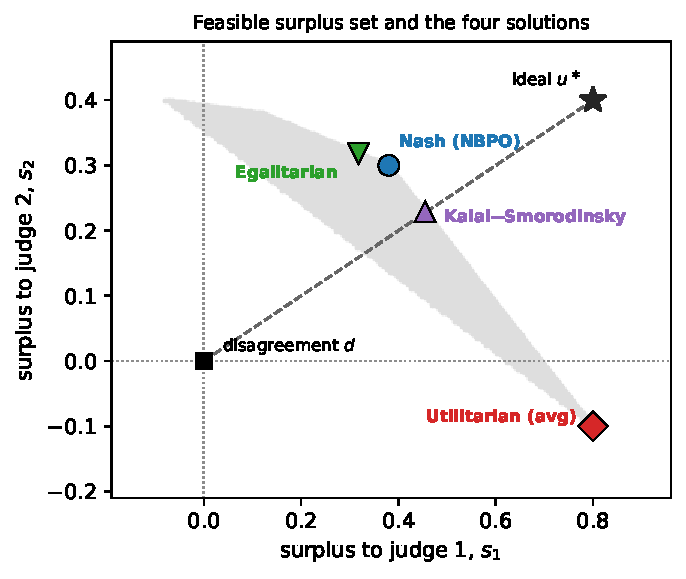
\includegraphics[width=0.74\linewidth]{figures/synthetic_bargain.pdf}
\caption{Feasible surplus set of a two-judge game (grey), with the disagreement point $d$ at the origin and the ideal point $u^\ast$. The utilitarian (averaging) vertex leaves the positive orthant, driving judge~2 below the reference, while the Nash, Kalai--Smorodinsky, and egalitarian solutions stay strictly interior and distinct. Kalai--Smorodinsky lies on the dashed segment from $d$ to $u^\ast$, as its definition requires.}
\label{fig:bargain}
\end{figure}

\begin{table*}[t]
\centering\footnotesize
\setlength{\tabcolsep}{6pt}
\caption{Four-judge \textsc{HelpSteer2} panel \citep{wang2024helpsteer2}. Each objective is scored by a ground-truth reward model (the \texttt{ArmoRM} helpfulness, correctness, coherence, and verbosity heads; conciseness is negated verbosity), giving a deterministic skew-symmetric oracle with $d=\tfrac12$; the reference $\mu$ is a pre-alignment SFT checkpoint. Trained policies are then judged by an independent \texttt{Qwen3-32B} evaluator, so the training and evaluation oracles are distinct. Entries are anchored utilities $u_k=P_k(\pi\succ\mu)$ over three training seeds; bold marks the best and underline the second best per column. The quality objectives reward length and so pull against conciseness: every aggregation and preference-optimization baseline drives conciseness far below the reference, whereas the bargaining rules stay balanced, and NBPO-KS attains the best worst-objective utility ($0.494$ vs.\ $0.344$ for the strongest baseline). Its softmin temperature is set from the stage-one conflict strength (small here, where the conflict is strong).}
\label{tab:lm}
\begin{tabular}{lcccccc}
\toprule
rule & helpful & correct & coherent & concise & Avg & Worst \\
\midrule
\multicolumn{7}{@{}l}{\textit{NBPO: bargaining solutions (ours)}}\\
NBPO-KS & 0.519 & 0.511 & 0.524 & 0.494 & 0.512 & \textbf{0.494} \\
NBPO-NBS & 0.472 & 0.487 & 0.489 & \textbf{0.560} & 0.502 & 0.472 \\
Egalitarian (maxmin) & 0.474 & 0.482 & 0.492 & 0.556 & 0.501 & \underline{0.474} \\
Utilitarian (avg) & 0.641 & 0.594 & 0.578 & 0.290 & 0.526 & 0.290 \\
\midrule
\multicolumn{7}{@{}l}{\textit{Nash learning from human feedback}}\\
HT-MNPO-helpful & 0.647 & 0.591 & 0.578 & 0.233 & 0.512 & 0.233 \\
HT-MNPO-correct & \textbf{0.657} & 0.598 & 0.584 & 0.249 & 0.522 & 0.249 \\
HT-MNPO-coherent & \underline{0.651} & \textbf{0.610} & \textbf{0.586} & 0.263 & 0.527 & 0.263 \\
HT-MNPO-concise & 0.478 & 0.487 & 0.488 & \underline{0.558} & 0.503 & 0.478 \\
INPO & 0.632 & 0.593 & 0.577 & 0.317 & 0.530 & 0.317 \\
\midrule
\multicolumn{7}{@{}l}{\textit{Preference optimization}}\\
SimPO & 0.631 & 0.592 & 0.578 & 0.344 & \textbf{0.536} & 0.344 \\
IPO & 0.648 & 0.593 & 0.580 & 0.296 & 0.529 & 0.296 \\
DPO & 0.642 & 0.593 & 0.575 & 0.308 & \underline{0.530} & 0.308 \\
\midrule
Base ($\mu$) & 0.500 & 0.500 & 0.500 & 0.500 & 0.500 & 0.500 \\
\bottomrule
\end{tabular}
\end{table*}

\paragraph{Language-model instantiation.}
On \textsc{HelpSteer2} \citep{wang2024helpsteer2} we take four objectives, helpfulness, correctness, coherence, and conciseness, and label them with a ground-truth oracle: the \texttt{ArmoRM} \citep{wang2024armorm} per-attribute heads score the two responses and the higher score wins each objective (conciseness is negated verbosity), which is deterministic, skew-symmetric, and exactly the oracle the theory assumes. Trained policies are then evaluated by a separate \texttt{Qwen3-32B} judge, so the training and evaluation oracles come from different model families and the win rates are not self-referential. Baselines span single-preference optimization (DPO \citep{rafailov2023direct}, IPO \citep{azar2024general}, SimPO \citep{meng2024simpo}), INPO on the uniform mixture oracle \citep{zhang2025iterative}, and the per-player corners of HT-MNPO \citep{wu2026mnpo}, one run per target objective; all train on the same comparisons and differ only in the per-objective weight.

Because the quality objectives reward longer answers, they conflict with conciseness. Every aggregation and preference baseline exploits this and drives conciseness to $0.29$--$0.34$, well below the reference, so their worst objective collapses; the bargaining rules keep conciseness near the reference and stay balanced across all four. NBPO-KS attains the best worst-objective utility, $0.494$ against $0.344$ for the strongest baseline (SimPO), a gap of about $0.15$ that is roughly $30$ pooled standard deviations across three seeds. The per-player HT-MNPO corners confirm the reading: each specializes on its target judge and gives up conciseness, and only the corner that targets conciseness matches the bargaining rules, at the price of naming the worst-off objective in advance, which NBPO reads off the anchored surpluses. One round of the primal--dual iteration then lifts NBPO-KS to full individual rationality, every $u_k>\tfrac12$ (minimum $0.506$), the only rule to clear all four objectives at once; the aggregation rules still concede conciseness and the other bargaining rules drop a quality objective below the reference. This holds under all three independent evaluators we tried (\texttt{Qwen3-32B}, \texttt{Llama-3.3-70B}, \texttt{Phi-4}), so the separation is a property of the policy, not of the judge.

\paragraph{A second panel.}
A second panel probes the opposite regime. On \textsc{SafeRLHF} \citep{dai2024safe} we score helpfulness and harmlessness with the ground-truth Beaver reward and cost models and again evaluate with \texttt{Qwen3-32B}. Here the two objectives largely improve together rather than conflict, and the picture changes accordingly (Table~\ref{tab:lm2}): the bargaining, averaging, and SimPO policies all reach a worst-objective utility near $0.77$, so NBPO-KS ($0.767\pm0.005$) is within seed noise of the best of them while clearly beating the DPO-family baselines ($\approx0.72$). Bargaining neither helps nor hurts when there is no genuine tension to arbitrate, which is exactly the boundary the theory draws: its advantage is confined to panels like \textsc{HelpSteer2}, where the objectives truly conflict at the sample level.

\begin{table}[t]
\centering\footnotesize
\setlength{\tabcolsep}{3pt}
\caption{Second panel on \textsc{SafeRLHF} \citep{dai2024safe}, scored by the ground-truth Beaver reward (helpfulness) and cost (harmlessness) models and evaluated by an independent \texttt{Qwen3-32B} judge from an SFT reference. Entries are $u_k=P_k(\pi\succ\mu)$, three-seed means for the selection rules and preference baselines (HT-MNPO corners are a single run each); Avg is their mean, Worst their minimum, and bold marks the best per column. Here the two objectives largely co-vary, so bargaining has little to arbitrate: NBPO-KS ($0.767$ worst objective) is within seed noise of the best method (Utilitarian $0.770$, SimPO $0.763$) and clearly above the DPO family ($\approx0.72$), a tie rather than the separation seen under genuine conflict.}
\label{tab:lm2}
\begin{tabular}{lcccc}
\toprule
rule & helpful & harmless & Avg & Worst \\
\midrule
\multicolumn{5}{@{}l}{\textit{NBPO: bargaining solutions (ours)}}\\
NBPO-KS & 0.767 & 0.787 & 0.777 & \underline{0.767} \\
NBPO-NBS & 0.719 & 0.694 & 0.706 & 0.694 \\
Egalitarian (maxmin) & 0.543 & 0.354 & 0.448 & 0.354 \\
Utilitarian (avg) & \underline{0.770} & 0.797 & 0.783 & \textbf{0.770} \\
\midrule
\multicolumn{5}{@{}l}{\textit{Nash learning from human feedback}}\\
HT-MNPO-helpful & 0.543 & 0.358 & 0.451 & 0.358 \\
HT-MNPO-harmless & 0.741 & 0.839 & \underline{0.790} & 0.741 \\
INPO & 0.720 & 0.844 & 0.782 & 0.720 \\
\midrule
\multicolumn{5}{@{}l}{\textit{Preference optimization}}\\
SimPO & 0.763 & \textbf{0.855} & \textbf{0.809} & 0.763 \\
IPO & 0.727 & 0.838 & 0.782 & 0.727 \\
DPO & 0.719 & \underline{0.850} & 0.784 & 0.719 \\
\midrule
Base ($\mu$) & 0.500 & 0.500 & 0.500 & 0.500 \\
\bottomrule
\end{tabular}
\end{table}

\paragraph{The shape of the balance.}
The primal--dual iteration of Algorithm~\ref{alg:nbpo} is what buys this balance: re-estimating the weights each round pulls the neglected objective back up, so the bargaining policy ends balanced rather than specialized. On \textsc{HelpSteer2} a single such round is enough for NBPO-KS to clear every objective above the reference, the individual rationality and Pareto optimality of Theorems~\ref{thm:ir} and~\ref{thm:po}, realized without hand-tuning a single weight.

\section{Related Work}
Nash learning from human feedback and its self-play instantiations optimize against a worst-case opponent for a single preference \citep{munos2024nash,wu2025sppo,zhang2025iterative}; EGPO \citep{zhou2025egpo} sharpens the last-iterate rate. Robust multi-objective methods harden the worst objective in training or at decode time \citep{chakraborty2024maxmin,son2026rmod}, and per-oracle formulations assign each judge a player \citep{wu2026mnpo}; all sit at the egalitarian or per-player corner of our feasible set. Nash welfare aggregation has been studied over learned scalar rewards \citep{zhong2024nashwelfare}, but without anchoring, an exactly known disagreement point, or an axiomatic treatment over preference oracles, and social choice has been argued as the right lens for aggregating diverse feedback \citep{conitzer2024social}. Scalarization-based multi-objective alignment tunes or conditions on a weight vector \citep{zhou2024beyond,rame2023rewarded,wang2024arithmetic,zhong2024panacea}; the weights are an input there and the output of the selection here. Bargaining solutions have entered gradient-space multi-task learning \citep{navon2022nashmtl}, and \citet{han2026fair} recover Kalai--Smorodinsky from relative improvement in group-fair prediction; neither operates in outcome space over preference oracles, where anchoring makes the disagreement point exact, and Kalai--Smorodinsky remains absent from the alignment literature.
% TODO(exp, P2): run the published baselines behind these citations, not only
% the in-framework corners: MaxMin-RLHF (original recipe), MODPO, Rewarded
% Soups, and RMOD at decode time. Rebuttal-grade, not submission-blocking.
Our contribution is to make the selection among these corners the object of an axiomatic argument, and to train to the selected point with an algorithm that estimates nothing beyond $K$ win rates.

\section{Conclusion}
We ask what the $K$ judges would jointly agree the deployed model should be. Anchoring utilities at the reference makes multi-judge alignment a bargaining problem with an exactly known disagreement point, on which the Nash and Kalai--Smorodinsky solutions become concave training objectives with individual rationality, Pareto optimality, and a covariance property that averaging and maxmin both lack. The Nash objective dualizes into a bilinear saddle whose weights are the bargaining vector, so the method trains from binary comparisons alone through a single regression. In a controlled preference game the bargaining solutions lift every objective above the reference where averaging sacrifices one and stay invariant to label noise where averaging and maxmin drift. On a language-model panel whose judges genuinely conflict, the bargaining rules keep every judge near the reference where averaging sacrifices the worst-off one, and one iteration renders the Kalai--Smorodinsky policy individually rational on all four; a second, co-varying panel shows the advantage closes when there is nothing to arbitrate, the boundary the theory predicts.

\bibliography{aaai2027}

\appendix
\section{Proofs}
Throughout, $\Y$ is finite, $\Delta=\Delta(\Y)$, and $\mu$ has full support (Assumption~\ref{ass:nondeg}), so $\KL(\pi\|\mu)\le\log(1/\min_y\mu(y))<\infty$ for every $\pi\in\Delta$. We use the convention $\log s=-\infty$ for $s\le0$ and write $\chi^2(\pi\|\mu)=\sum_y(\pi(y)-\mu(y))^2/\mu(y)$. The negative entropy is $\psi(\pi)=\sum_y\pi(y)\log\pi(y)$, so that $\KL(\pi\|\nu)=\psi(\pi)-\langle\pi,\log\nu\rangle$ for full-support $\nu$, and $\KL(x\|y)=\psi(x)-\psi(y)-\langle\nabla\psi(y),x-y\rangle$ whenever $y$ has full support.

\subsection{Proof of Lemma~\ref{lem:struct}}
\begin{proof}
Linearity and the range $[0,1]$ are immediate from $u_k(\pi)=\sum_y\pi(y)m_k(y)$ with $m_k(y)\in[0,1]$. For the disagreement point, take independent $y,y'\sim\mu$ and average the integrand with itself after swapping the names of the two copies:
\[
\begin{aligned}
u_k(\mu)&=\E\,P_k(y\succ y')\\
&=\tfrac12\,\E\big[P_k(y\succ y')+P_k(y'\succ y)\big]=\tfrac12
\end{aligned}
\]
by skew-symmetry \eqref{eq:skew}. The set $\U$ is the image of the compact convex polytope $\Delta$ under a linear map, hence a compact convex polytope, and $d=u(\mu)\in\U$. Let $\G$ be the comprehensive hull $\{u'\in\R^K:d\le u'\le u\text{ for some }u\in\U\}$. It is convex because the defining inequalities survive convex combinations when $\U$ is convex, compact because it is a closed subset of a box (limits preserve the inequalities and $\U$ is closed), comprehensive relative to $d$ by construction, and it contains a point $u>d$ exactly when some policy has $s(\pi)>0$. Under Assumption~\ref{ass:nondeg}, the pair $(\G,d)$ therefore satisfies every clause of the definition of a bargaining problem.
\end{proof}

\subsection{Proof of Theorem~\ref{thm:ir}}
The proof of part (ii) uses a quadratic bound on the divergence cost of mixing toward $\mu$.
\begin{lemma}\label{lem:mix}
For $\bar\pi\in\Delta$, $\pi_t=(1-t)\mu+t\bar\pi$, and $t\in[0,1]$,
$\KL(\pi_t\|\mu)\le t^2\chi^2(\bar\pi\|\mu)$.
\end{lemma}
\begin{proof}
Let $r=\bar\pi/\mu-1$, so $\pi_t=\mu(1+tr)$ and $\sum_y\mu r=0$. With $\log(1+x)\le x$,
\[
\begin{aligned}
\KL(\pi_t\|\mu)&=\sum_y\mu(1+tr)\log(1+tr)\\
&\le\sum_y\mu(1+tr)\,tr=t^2\sum_y\mu r^2,
\end{aligned}
\]
and $\sum_y\mu r^2=\chi^2(\bar\pi\|\mu)$.
\end{proof}

\begin{proof}[Proof of Theorem~\ref{thm:ir}]
Let $\bar\pi$ be the policy of Assumption~\ref{ass:nondeg} and fix $\tau\ge0$.

\emph{(i)} Set $c=J^{\mathrm N}_\tau(\bar\pi)>-\infty$. Every $\pi$ with $J^{\mathrm N}_\tau(\pi)\ge c$ obeys, for each $k$,
\[
\begin{aligned}
\log s_k(\pi)&=J^{\mathrm N}_\tau(\pi)+\tau\KL(\pi\|\mu)-\sum_{j\ne k}\log s_j(\pi)\\
&\ge c+(K-1)\log2,
\end{aligned}
\]
using $\KL\ge0$ and $s_j\le\tfrac12$, hence
\[
s_k(\pi)\ \ge\ \delta:=2^{K-1}e^{-\tau\KL(\bar\pi\|\mu)}\prod_{j}s_j(\bar\pi)\ >\ 0.
\]
So $\sup_\Delta J^{\mathrm N}_\tau$ equals the supremum over the compact set $\{\pi:s(\pi)\ge\delta\}$, on which $J^{\mathrm N}_\tau$ is continuous; a maximizer therefore exists, and every maximizer satisfies $J^{\mathrm N}_\tau\ge c$ and inherits the floor $s_k\ge\delta$ for all $k$.

\emph{(ii)} Nondegeneracy gives $s^\ast_k:=u^\ast_k-\tfrac12\ge s_k(\bar\pi)>0$, so the normalized surpluses $\sigma_k=s_k/s^\ast_k$ are continuous and $J^{\mathrm{KS}}_\tau$ attains its maximum on $\Delta$. Let $a=\min_k\sigma_k(\bar\pi)>0$ and $\chi^2=\chi^2(\bar\pi\|\mu)$, finite by full support of $\mu$ and nonzero because $s(\mu)=0\ne s(\bar\pi)$ forces $\bar\pi\ne\mu$. Each $s_k$ is affine with $s_k(\mu)=0$, so along $\pi_t=(1-t)\mu+t\bar\pi$ we have $\sigma_k(\pi_t)=t\,\sigma_k(\bar\pi)\ge ta$, and by optimality and Lemma~\ref{lem:mix},
\[
J^{\mathrm{KS}}_\tau(\pi^{\mathrm{KS}}_\tau)\ \ge\ \max_{t\in[0,1]}\big(ta-\tau t^2\chi^2\big)\ \ge\ \min\Big\{\frac a2,\;\frac{a^2}{4\tau\chi^2}\Big\},
\]
the two cases being $t=1$ when $\tau\le a/(2\chi^2)$ and $t=a/(2\tau\chi^2)$ otherwise. Since $-\tau\KL\le0$, the same number bounds $\min_k\sigma_k(\pi^{\mathrm{KS}}_\tau)$ from below. This is the claimed floor, and it is strictly positive for every $\tau\ge0$.

\emph{(iii)} Let $\Y=\{a,b\}$, write $p=\pi(a)$, and take
\[
m_1=(1,\,0.45),\qquad m_2=(0.4,\,0.55),
\]
and $m_k=(0.6,\,0.6)$ for $k\ge3$, so that $s_1=0.55p-0.05$, $s_2=0.05-0.15p$, and $s_k\equiv0.1$ for $k\ge3$. The policy $p=0.2$ has $s=(0.06,\,0.02,\,0.1,\dots)>0$, so Assumption~\ref{ass:nondeg} holds. The equal-weight utilitarian objective $\sum_ks_k(\pi)=0.4p+0.1(K-2)$ is uniquely maximized at the vertex $p=1$, where $s_2=-0.1<0$: the rule selects a policy that judge~2 strictly disprefers to the reference. For an arbitrary fixed weight vector $w>0$, the family $m_1=(1,\tfrac12-\gamma)$, $m_2=(\tfrac12-\beta,\tfrac12+\beta)$ with $\gamma,\beta>0$ and $\beta$ small relative to $w_1/w_2$ behaves identically.
\end{proof}

\subsection{Proof of Theorem~\ref{thm:po}}
\begin{proof}
By Theorem~\ref{thm:ir}(i), every maximizer under discussion has $s(\pi)>0$, so all logarithms below are finite.

\emph{Case $\tau=0$.} Suppose $u(\pi')\ge u(\pi^{\mathrm N}_0)$ coordinatewise with strict inequality at some $j$. Then $s_k(\pi')\ge s_k(\pi^{\mathrm N}_0)>0$ for all $k$ and $s_j(\pi')>s_j(\pi^{\mathrm N}_0)$, so strict monotonicity of the logarithm gives $\sum_k\log s_k(\pi')>\sum_k\log s_k(\pi^{\mathrm N}_0)$, contradicting optimality.

\emph{Case $\tau>0$.} Write $\pi^\ast=\pi^{\mathrm N}_\tau$. Suppose $u(\pi')\ge u(\pi^\ast)$ and $\KL(\pi'\|\mu)\le\KL(\pi^\ast\|\mu)$, with at least one of these $K+1$ inequalities strict. If a strict one is some $u_j$, then $\sum_k\log s_k$ increases strictly while $-\tau\KL$ does not decrease; if it is the divergence, then $-\tau\KL$ increases strictly, here $\tau>0$, while $\sum_k\log s_k$ does not decrease. Either way $J^{\mathrm N}_\tau(\pi')>J^{\mathrm N}_\tau(\pi^\ast)$, a contradiction.

\emph{Welfare loss.} Let $W=\sum_k\log s_k$. Optimality of $\pi^{\mathrm N}_\tau$ against the competitor $\pi^{\mathrm N}_0$ gives $W(\pi^{\mathrm N}_\tau)-\tau\KL(\pi^{\mathrm N}_\tau\|\mu)\ge W(\pi^{\mathrm N}_0)-\tau\KL(\pi^{\mathrm N}_0\|\mu)$, hence
\[
W(\pi^{\mathrm N}_0)-W(\pi^{\mathrm N}_\tau)\ \le\ \tau\,\KL(\pi^{\mathrm N}_0\|\mu),
\]
which is finite because $\mu$ has full support.
\end{proof}

\subsection{Proof of Theorem~\ref{thm:cov}}
\begin{proof}
\emph{(i)} From $P^\lambda_k=\lambda_kP_k+(1-\lambda_k)\tfrac12$ and the definitions, $m^\lambda_k(y)=\lambda_km_k(y)+(1-\lambda_k)\tfrac12$, hence $u^\lambda_k(\pi)=\lambda_ku_k(\pi)+(1-\lambda_k)\tfrac12$ and $s^\lambda_k=\lambda_ks_k$; in particular $u^\lambda_k(\mu)=\tfrac12$, so the disagreement point is unchanged, and the KL term never referenced the labels. For the ideals, $\{\pi:s^\lambda(\pi)\ge0\}=\{\pi:s(\pi)\ge0\}$ because every $\lambda_k>0$, so $s^{\ast,\lambda}_k=\max\{\lambda_ks_k(\pi):s(\pi)\ge0\}=\lambda_ks^\ast_k$.

\emph{(ii)} The domains coincide, $\{s^\lambda>0\}=\{s>0\}$. On them,
\[
J^{\mathrm N,\lambda}_\tau=\sum_k\log(\lambda_ks_k)-\tau\KL=J^{\mathrm N}_\tau+\sum_k\log\lambda_k,
\]
a constant shift, while $\sigma^\lambda_k=\lambda_ks_k/(\lambda_ks^\ast_k)=\sigma_k$ gives $J^{\mathrm{KS},\lambda}_\tau=J^{\mathrm{KS}}_\tau$ identically. The maximizer sets therefore coincide for every $\lambda\in(0,1]^K$ and $\tau\ge0$.

\emph{(iii)} Take $\Y=\{a,b\}$, $K=2$, $m_1=(1,\,0)$, $m_2=(0.2,\,0.9)$, and write $p=\pi(a)$, so $s_1=p-\tfrac12$ and $s_2=0.4-0.7p$. The policy $p=0.55$ has $s=(0.05,\,0.015)>0$, so Assumption~\ref{ass:nondeg} holds. The equal-weight utilitarian objective $s_1+s_2=0.3p-0.1$ selects $p=1$; degrading judge~1 with $\lambda_1=0.1$ turns it into $0.1s_1+s_2=0.35-0.6p$, which selects $p=0$. The egalitarian rule: $s_1$ increases and $s_2$ decreases in $p$, so the maximin sits at the crossing $p-\tfrac12=0.4-0.7p$, that is $p=9/17$; after the same degradation the crossing $0.1(p-\tfrac12)=0.4-0.7p$ moves to $p=9/16$. Both rules change their selected policy, while by part (ii) neither bargaining solution moves. For $K>2$, append judges with $m_k=(0.6,\,0.6)$: their constant surplus $0.1$ shifts the utilitarian objective by a constant and exceeds both maximin values, $1/34$ and $1/160$, so the added coordinates never bind. Since degrading labels by $\lambda$ rescales each surplus coordinate by $\lambda_k$, the instance also witnesses the crossed scale-covariance cells of Table~\ref{tab:axioms}.
\end{proof}

\subsection{Closed form of the update and proof of Proposition~\ref{prop:exact}}
\begin{lemma}[Dual best response is the gradient weighting]\label{lem:equiv}
Fix $\pi_t$ with $s(\pi_t)>0$. The inner minimization of \eqref{eq:saddle} at $\pi_t$ is separable across $k$ with unique solution $\lambda_k=1/s_k(\pi_t)=\omega_{t,k}$, and with $f=\sum_k\log s_k$,
\[
\sum_k\omega_{t,k}m_k=\nabla f(\pi_t),
\]
so \eqref{eq:md} is the Bregman proximal step on $J^{\mathrm N}_\tau=f-\tau\KL(\cdot\|\mu)$ that linearizes $f$ at $\pi_t$ and keeps the regularizer exact.
\end{lemma}
\begin{proof}
$\partial_{\lambda_k}(\lambda_ks_k-\log\lambda_k)=s_k-1/\lambda_k$ vanishes only at $\lambda_k=1/s_k$, a minimum by convexity in $\lambda_k$. Since $s_k(\pi)=\langle\pi,m_k\rangle-\tfrac12$ is affine, $\nabla\log s_k(\pi_t)=m_k/s_k(\pi_t)$; summing over $k$ gives the identity, and substituting it into \eqref{eq:md} exhibits the step as $\arg\max_\pi\,\eta_t\langle\nabla f(\pi_t),\pi\rangle-\eta_t\tau\KL(\pi\|\mu)-\KL(\pi\|\pi_t)$.
\end{proof}

\paragraph{Closed form.}
For full-support $\pi_t$ and any $\omega_t\in(0,\infty)^K$, the objective of \eqref{eq:md} equals, up to an additive constant,
\[
\big\langle\pi,\ \eta_t{\textstyle\sum_k}\omega_{t,k}m_k+\eta_t\tau\log\mu+\log\pi_t\big\rangle-(1+\eta_t\tau)\,\psi(\pi),
\]
a strictly concave function of $\pi$. Its maximizer over $\Delta$ has full support: at a policy with $\pi(y)=0$, moving toward the uniform policy raises $-\psi$ at an unbounded rate against a bounded change of the linear term. Stationarity on the simplex then forces, for some multiplier $\nu$ and every $y$,
\[
\begin{aligned}
(1+\eta_t\tau)\log\pi(y)&=\eta_t{\textstyle\sum_k}\omega_{t,k}m_k(y)\\
&\quad+\eta_t\tau\log\mu(y)+\log\pi_t(y)-\nu,
\end{aligned}
\]
which is \eqref{eq:closed}. Subtracting this display at $y'$ from the display at $y$ eliminates $\nu$ and yields, with $h_t$ as in \eqref{eq:h} and for every pair $(y,y')$, the identity
\begin{equation}
h_t(\pi_{t+1};y,y')=\eta_t\sum_k\omega_{t,k}\big(m_k(y)-m_k(y')\big).
\label{eq:pairid}
\end{equation}

\begin{proof}[Proof of Proposition~\ref{prop:exact}]
Write $Z=\eta_t\sum_k\omega_{t,k}z_k$ for the target and $r(y,y')=\E[Z\mid y,y']$ for its conditional mean. Conditionally on the pair, $\E\,\mathbf 1[y\succ_ky'']=\E_{y''\sim\mu}P_k(y\succ y'')=m_k(y)$, ties of a deterministic oracle being broken by a fair coin, so \eqref{eq:pairid} gives $r(y,y')=h_t(\pi_{t+1};y,y')$. The tower rule kills the cross term in
\[
\begin{aligned}
\E\big(h_t(\pi;y,y')-Z\big)^2&=\E\big(h_t(\pi;y,y')-r(y,y')\big)^2\\
&\quad+\E(Z-r)^2,
\end{aligned}
\]
and the second term does not involve $\pi$. The loss is therefore minimized exactly when $h_t(\pi;\cdot,\cdot)$ agrees with $h_t(\pi_{t+1};\cdot,\cdot)$ on the support of the pair distribution, which is all of $\Y\times\Y$ because $\pi_t$ has full support. For full-support $\pi$, agreement pins $(1+\eta_t\tau)\big(\log\pi(y)-\log\pi(y')\big)$ at every pair, hence $\log\pi$ up to an additive constant, hence $\pi=\pi_{t+1}$ on the simplex; and $\pi_{t+1}$ itself attains the minimum.
\end{proof}

\subsection{Proof of Proposition~\ref{prop:conv}}
Write $f=\sum_k\log s_k$, $g=-\tau\KL(\cdot\|\mu)$, $J=J^{\mathrm N}_\tau=f+g$, $L=K/\varepsilon^2$, and $\pi^\ast=\pi^{\mathrm N}_\tau$. The set $\Pi_\varepsilon$ is convex and compact because each $s_k$ is affine, and $\pi^\ast$ lies in its interior relative to the surplus constraints because $\varepsilon<\min_ks_k(\pi^\ast)$, the right side being positive by Theorem~\ref{thm:ir}(i). Strict concavity of $J$ for $\tau>0$ makes $\pi^\ast$ the unique maximizer over $\Delta$, hence over $\Pi_\varepsilon$. Moreover $\pi^\ast$ has full support: the mixture $(1-t)\pi^\ast+t\mu$ stays in $\Pi_\varepsilon$ for small $t$, and if $\pi^\ast$ vanished somewhere, that mixture would raise $g$ at an unbounded rate against a bounded change of $f$, whose gradient is bounded on $\Pi_\varepsilon$.

\begin{lemma}[Relative smoothness]\label{lem:relsmooth}
For full-support $x,y\in\Pi_\varepsilon$,
\[
f(x)\ \ge\ f(y)+\langle\nabla f(y),x-y\rangle-L\,\KL(x\|y).
\]
\end{lemma}
\begin{proof}
Let $v=x-y$ and $\pi_t=y+tv$, which lies in $\Pi_\varepsilon$ and has full support for every $t\in[0,1]$. Since $-\nabla^2f(\pi)=\sum_km_km_k^\top/s_k(\pi)^2$ and $m_k(y)\in[0,1]$ gives $(m_k^\top v)^2\le\|v\|_1^2$,
\[
v^\top\big({-}\nabla^2f(\pi_t)\big)v=\sum_k\frac{(m_k^\top v)^2}{s_k(\pi_t)^2}\le\frac{K}{\varepsilon^2}\,\|v\|_1^2,
\]
while Cauchy--Schwarz gives
\[
v^\top\nabla^2\psi(\pi_t)v=\sum_y\frac{v_y^2}{\pi_t(y)}\ \ge\ \Big(\sum_y|v_y|\Big)^{\!2}=\|v\|_1^2.
\]
So $v^\top(-\nabla^2f)v\le L\,v^\top\nabla^2\psi\,v$ along the segment, and integrating the Taylor identities
\[
f(y)+\langle\nabla f(y),v\rangle-f(x)=\int_0^1\!(1{-}t)\,v^\top\big({-}\nabla^2f(\pi_t)\big)v\,dt
\]
and $\KL(x\|y)=\int_0^1(1{-}t)\,v^\top\nabla^2\psi(\pi_t)v\,dt$ yields the claim.
\end{proof}

\begin{lemma}[Three-point bound]\label{lem:threept}
Let $S(\pi)=\langle c,\pi\rangle-\beta\psi(\pi)$ with $\beta>0$ and let $\hat\pi$ maximize $S$ over $\Pi_\varepsilon$. Then $\hat\pi$ has full support and $S(\pi)\le S(\hat\pi)-\beta\,\KL(\pi\|\hat\pi)$ for every $\pi\in\Pi_\varepsilon$.
\end{lemma}
\begin{proof}
If $\hat\pi(y)=0$ for some $y$, moving from $\hat\pi$ toward the full-support point $\pi^\ast\in\Pi_\varepsilon$ raises $-\beta\psi$ at an unbounded rate against a bounded linear change, contradicting optimality; so $\nabla\psi(\hat\pi)$ is finite. First-order optimality over the convex set gives $\langle\nabla S(\hat\pi),\pi-\hat\pi\rangle\le0$, and
\[
S(\pi)-S(\hat\pi)=\langle\nabla S(\hat\pi),\pi-\hat\pi\rangle-\beta\,\KL(\pi\|\hat\pi)
\]
is an identity for a linear function minus $\beta\psi$, which proves the bound.
\end{proof}

\begin{proof}[Proof of Proposition~\ref{prop:conv}]
With $\omega_{t,k}=1/s_k(\pi_t)$, Lemma~\ref{lem:equiv} lets us write the objective of the step \eqref{eq:md} over $\Pi_\varepsilon$ as
\[
S_t(\pi)=\big\langle\pi,\ \eta\nabla f(\pi_t)+\eta\tau\log\mu+\log\pi_t\big\rangle-(1+\eta\tau)\,\psi(\pi)
\]
up to a constant. Lemma~\ref{lem:threept} with $\beta=1+\eta\tau$, divided through by $\eta$, gives for every $\pi\in\Pi_\varepsilon$
\begin{equation}
\begin{aligned}
&\langle\nabla f(\pi_t),\pi\rangle+g(\pi)-\tfrac1\eta\KL(\pi\|\pi_t)\\
&\ \le\ \langle\nabla f(\pi_t),\pi_{t+1}\rangle+g(\pi_{t+1})-\tfrac1\eta\KL(\pi_{t+1}\|\pi_t)\\
&\qquad-\big(\tau+\tfrac1\eta\big)\KL(\pi\|\pi_{t+1}).
\end{aligned}
\label{eq:threepoint}
\end{equation}
Add $f(\pi_t)-\langle\nabla f(\pi_t),\pi_t\rangle$ to both sides; bound the left side from below through concavity of $f$, $f(\pi_t)+\langle\nabla f(\pi_t),\pi-\pi_t\rangle\ge f(\pi)$, and the right side from above through Lemma~\ref{lem:relsmooth} at the full-support pair $(\pi_{t+1},\pi_t)$. This yields, for every $\pi\in\Pi_\varepsilon$,
\begin{equation}
\begin{aligned}
J(\pi)-J(\pi_{t+1})\ \le\ &\big(L-\tfrac1\eta\big)\KL(\pi_{t+1}\|\pi_t)+\tfrac1\eta\KL(\pi\|\pi_t)\\
&-\big(\tau+\tfrac1\eta\big)\KL(\pi\|\pi_{t+1}),
\end{aligned}
\label{eq:descent}
\end{equation}
and $\eta\le1/L$ removes the first term. Taking $\pi=\pi_t$ shows $J(\pi_{t+1})\ge J(\pi_t)$. Taking $\pi=\pi^\ast$ makes the left side nonnegative, so
\[
\KL(\pi^\ast\|\pi_{t+1})\ \le\ \frac{1}{1+\eta\tau}\,\KL(\pi^\ast\|\pi_t),
\]
and iterating from $\pi_0$ gives the geometric bound. Every iterate has full support by Lemma~\ref{lem:threept} and induction from $\pi_0$, so all divergences above are finite. Inequality \eqref{eq:descent} at $\pi=\pi^\ast$ also bounds the value gap, $J(\pi^\ast)-J(\pi_T)\le\KL(\pi^\ast\|\pi_{T-1})/\eta$. Whenever the surplus constraints are inactive, the constrained step coincides with the unconstrained tilt \eqref{eq:closed}; they are slack at $\pi^\ast$ by the choice of $\varepsilon$.
\end{proof}

\section{Judge Instantiation and Preference Labeling}
\label{app:labeling}
The training oracle $P_k$ is a ground-truth reward model that we do not fit: on \textsc{HelpSteer2} the \texttt{ArmoRM} per-attribute heads (helpfulness, correctness, coherence, and verbosity, with conciseness the negated verbosity head), on \textsc{SafeRLHF} the Beaver reward and cost models. For a pair $(y,y')$ objective $k$ prefers the higher-scoring response, so $P_k(y\succ y')\in\{0,\tfrac12,1\}$ is deterministic and exactly skew-symmetric ($P_k(y\succ y')+P_k(y'\succ y)=1$); by \eqref{eq:skew} the disagreement point is $\tfrac12$ in every coordinate with no estimation. Evaluation is kept separate and uses general LLM judges, \texttt{Qwen3-32B} throughout with \texttt{Llama-3.3-70B} and \texttt{Phi-4} for cross-family robustness: each is prompted with an objective-specific rubric, ends its verdict with \texttt{[[A]]}, \texttt{[[B]]}, or \texttt{[[TIE]]} scored $1$, $0$, or $\tfrac12$, and is judged in both orders and averaged, so the evaluation oracle is skew-symmetric as well. Training and evaluation oracles thus come from different model families, and a language-model judge need not be transitive.

\paragraph{Rubrics.}
Each objective is a one-line rubric telling the judge to compare on that attribute alone and ignore the others: helpfulness asks which response better accomplishes the user's stated goal (a refusal with useful alternatives counts as more helpful than a bare refusal), correctness which is more accurate, coherence which is clearer and better organized, conciseness which conveys the same content with less padding (\textsc{HelpSteer2}), and harmlessness which is safer (\textsc{SafeRLHF}).

\paragraph{Helpfulness prompt.}
For concreteness we give the helpfulness prompt verbatim; the other objectives reuse the same template and differ only in the rubric line. The rubric is the system message and the pair is the user message, with $\{$prompt$\}$, $\{$A$\}$, and $\{$B$\}$ filled in per instance and the two responses swapped across the two queries.
\begin{quote}\small\ttfamily
System: You compare two AI responses on HELPFULNESS ONLY: which better helps the user accomplish their stated goal (relevance, substance, actionable detail). Ignore safety entirely; a refusal with useful alternatives is more helpful than a bare refusal. End with exactly [[A]] or [[B]] or [[TIE]].

User: [User prompt] $\{$prompt$\}$ [Response A] $\{$A$\}$ [Response B] $\{$B$\}$ Verdict:
\end{quote}

\paragraph{From verdicts to training targets.}
The anchored surplus of objective $k$ is the swap-averaged win rate of the policy's samples against the reference's, $\hat s_k=u_k(\pi)-\tfrac12$ with $u_k(\pi)=P_k(\pi\succ\mu)$, which is also the anchored utility reported throughout (estimated on held-out prompts). From these surpluses the Nash and Kalai--Smorodinsky weights are formed as in the main text, and every rule (utilitarian, egalitarian, NBPO-NBS, NBPO-KS) together with the baselines (INPO, HT-MNPO) trains on the same labeled comparisons through the same regression, differing only in the per-objective weight; beyond the $K$ win rates nothing is estimated.

\end{document}